\subsection{Vibrational action spectroscopy}
\label{subsec:action:methods:vibrational}

Photodissociation of isolated ions after light absorption (as long as the energy of the absorbed photons is higher than the bond dissociation threshold) is likely one of the most straightforward experimental techniques. So, most gas-phase action ion spectroscopy methods rely on the detection of charged products of dissociation or the loss of the parent ion signal after one or more photons are absorbed. In 1973, \citet{dunbar_photodissociation_1973} first investigated photodissociation in the visible spectral range. Soon after, \citet{okumura_vibrational_1985} studied photodissociation in the infrared region yielding the vibrational spectra.

In general, a single IR photon's absorption is insufficient to promote the breakdown of covalent bonds. However, several ways to circumvent this constraint are described in the following sections.

\subsubsection{Tagging photodissociation ion spectroscopy}
\label{subsec:action:methods:vibrational:IRPD}
The most straightforward technique to overcome the limitation is to utilise a loosely bound \qt{tag} to the molecular ion that detaches upon absorption of a single IR photon. The tags are chosen to have minimal effect on the structure of the ion core, i.e., they should be very weakly bound. Therefore, rare gas atoms such as He, Ne or Ar are preferred tagging agents.

The formed weakly bound complexes are dissociated as a result of resonance photon absorption as shown in Figure \ref{fig:IRPD} and the vibrational spectra are recorded as a function of IR frequency as shown in Figure \ref{fig:IRPD_spectrum}. This process is known as \qt{photo-dissociation} or \qt{pre-dissociation}. The very well-known technique using this approach for measuring vibrational transitions is called \qt{\textbf{I}nfra\textbf{R}ed \textbf{P}hoto-\textbf{D}issociation} (IRPD) spectroscopy.

\begin{figure}[!htb]
    \centering
    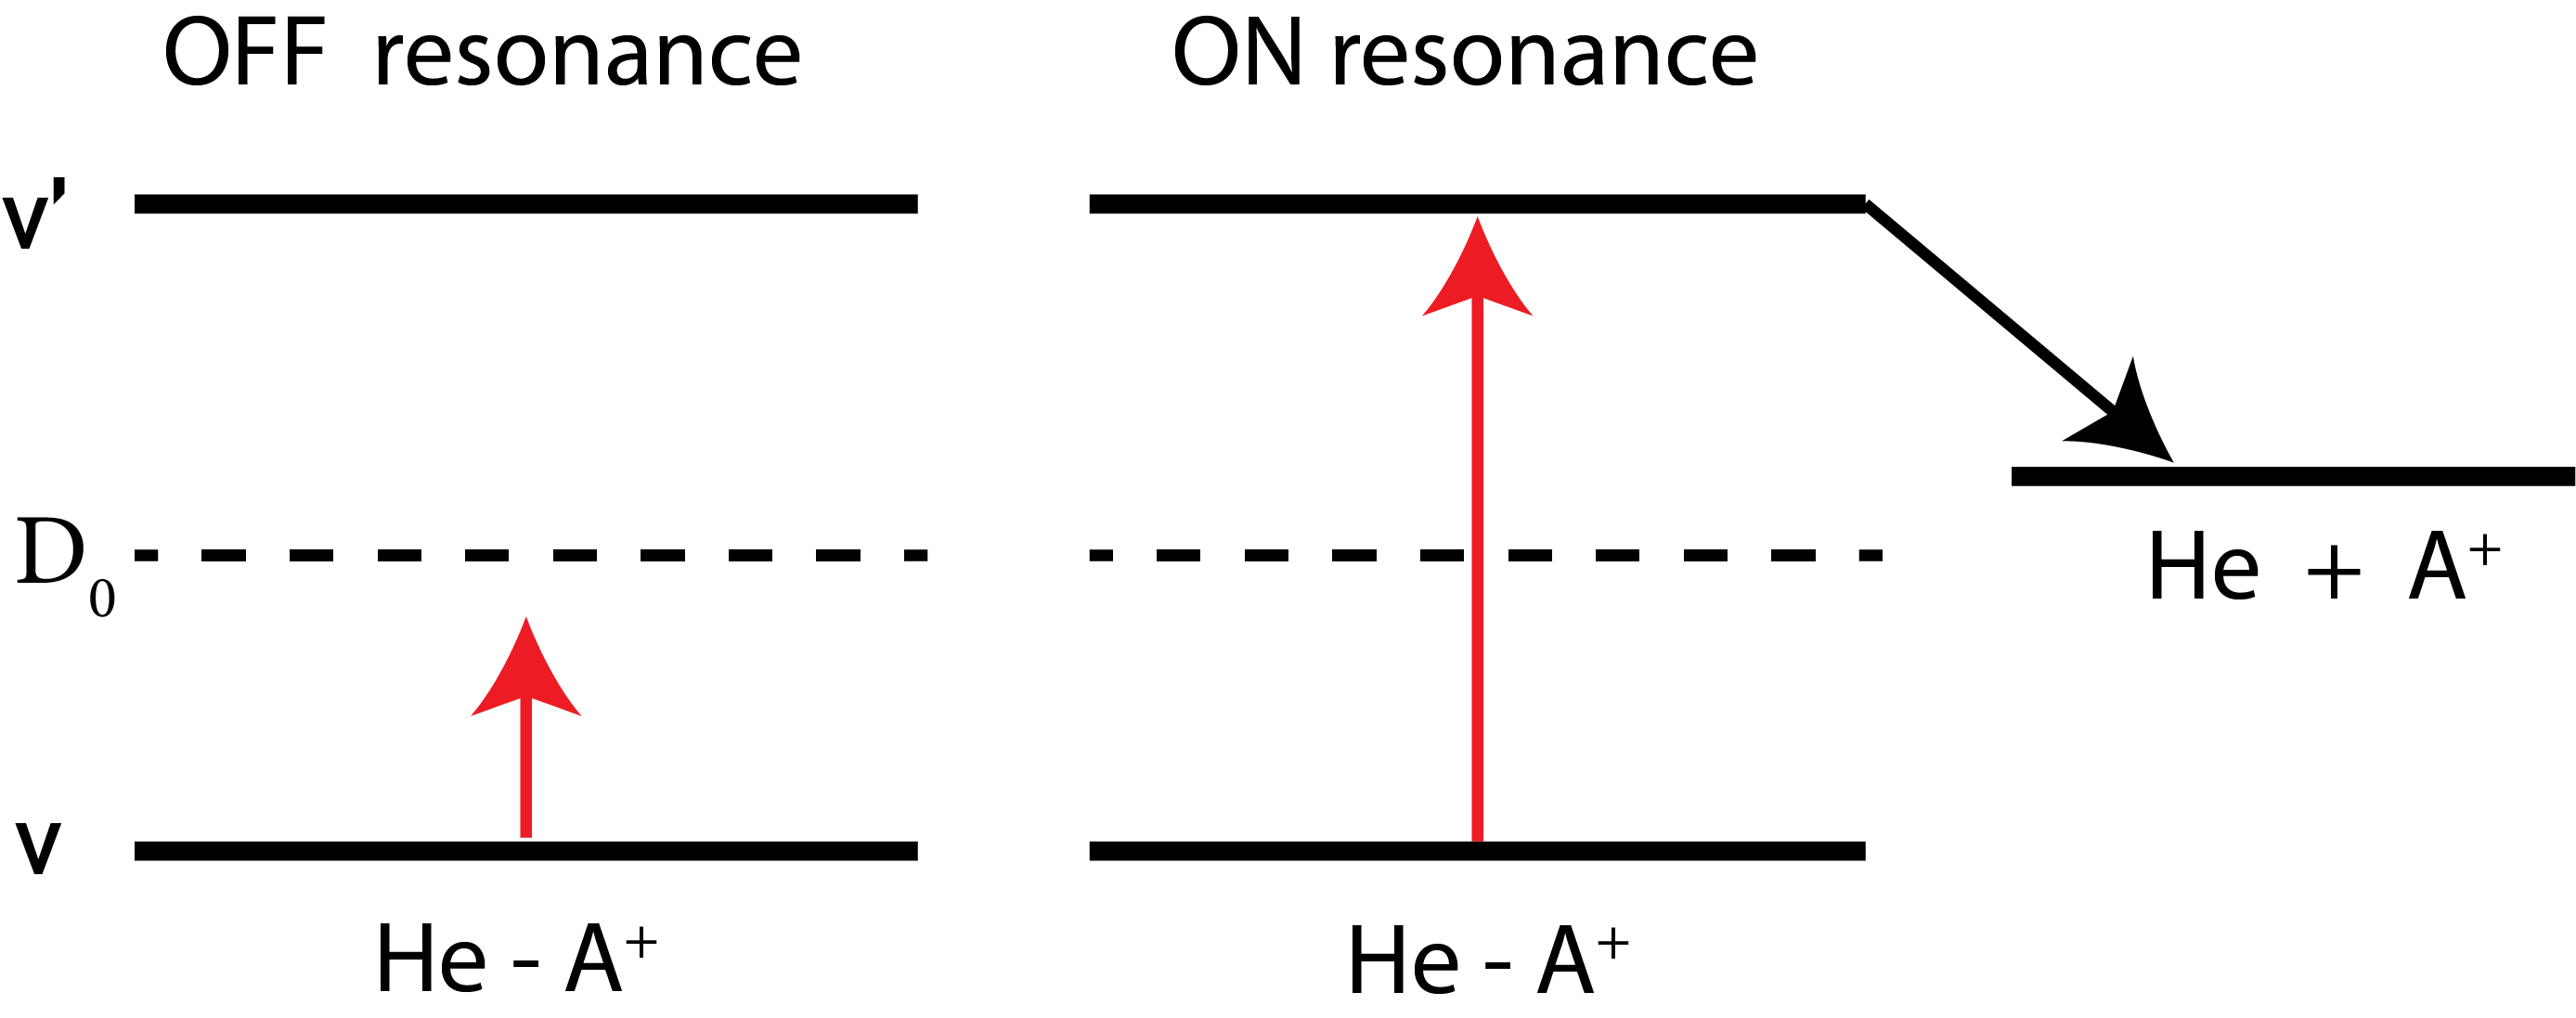
\includegraphics[width=0.9\textwidth]{figures/intro/IRPD.png}
    \caption{Schematic drawing of the IRPD method. He$-$A$^+$ represents the weakly bound helium complex of molecular ion A$^+$, and D$_0$ indicates the complex dissociation limit.}
    \label{fig:IRPD}
\end{figure}

\begin{figure}[!htb]
    \centering
    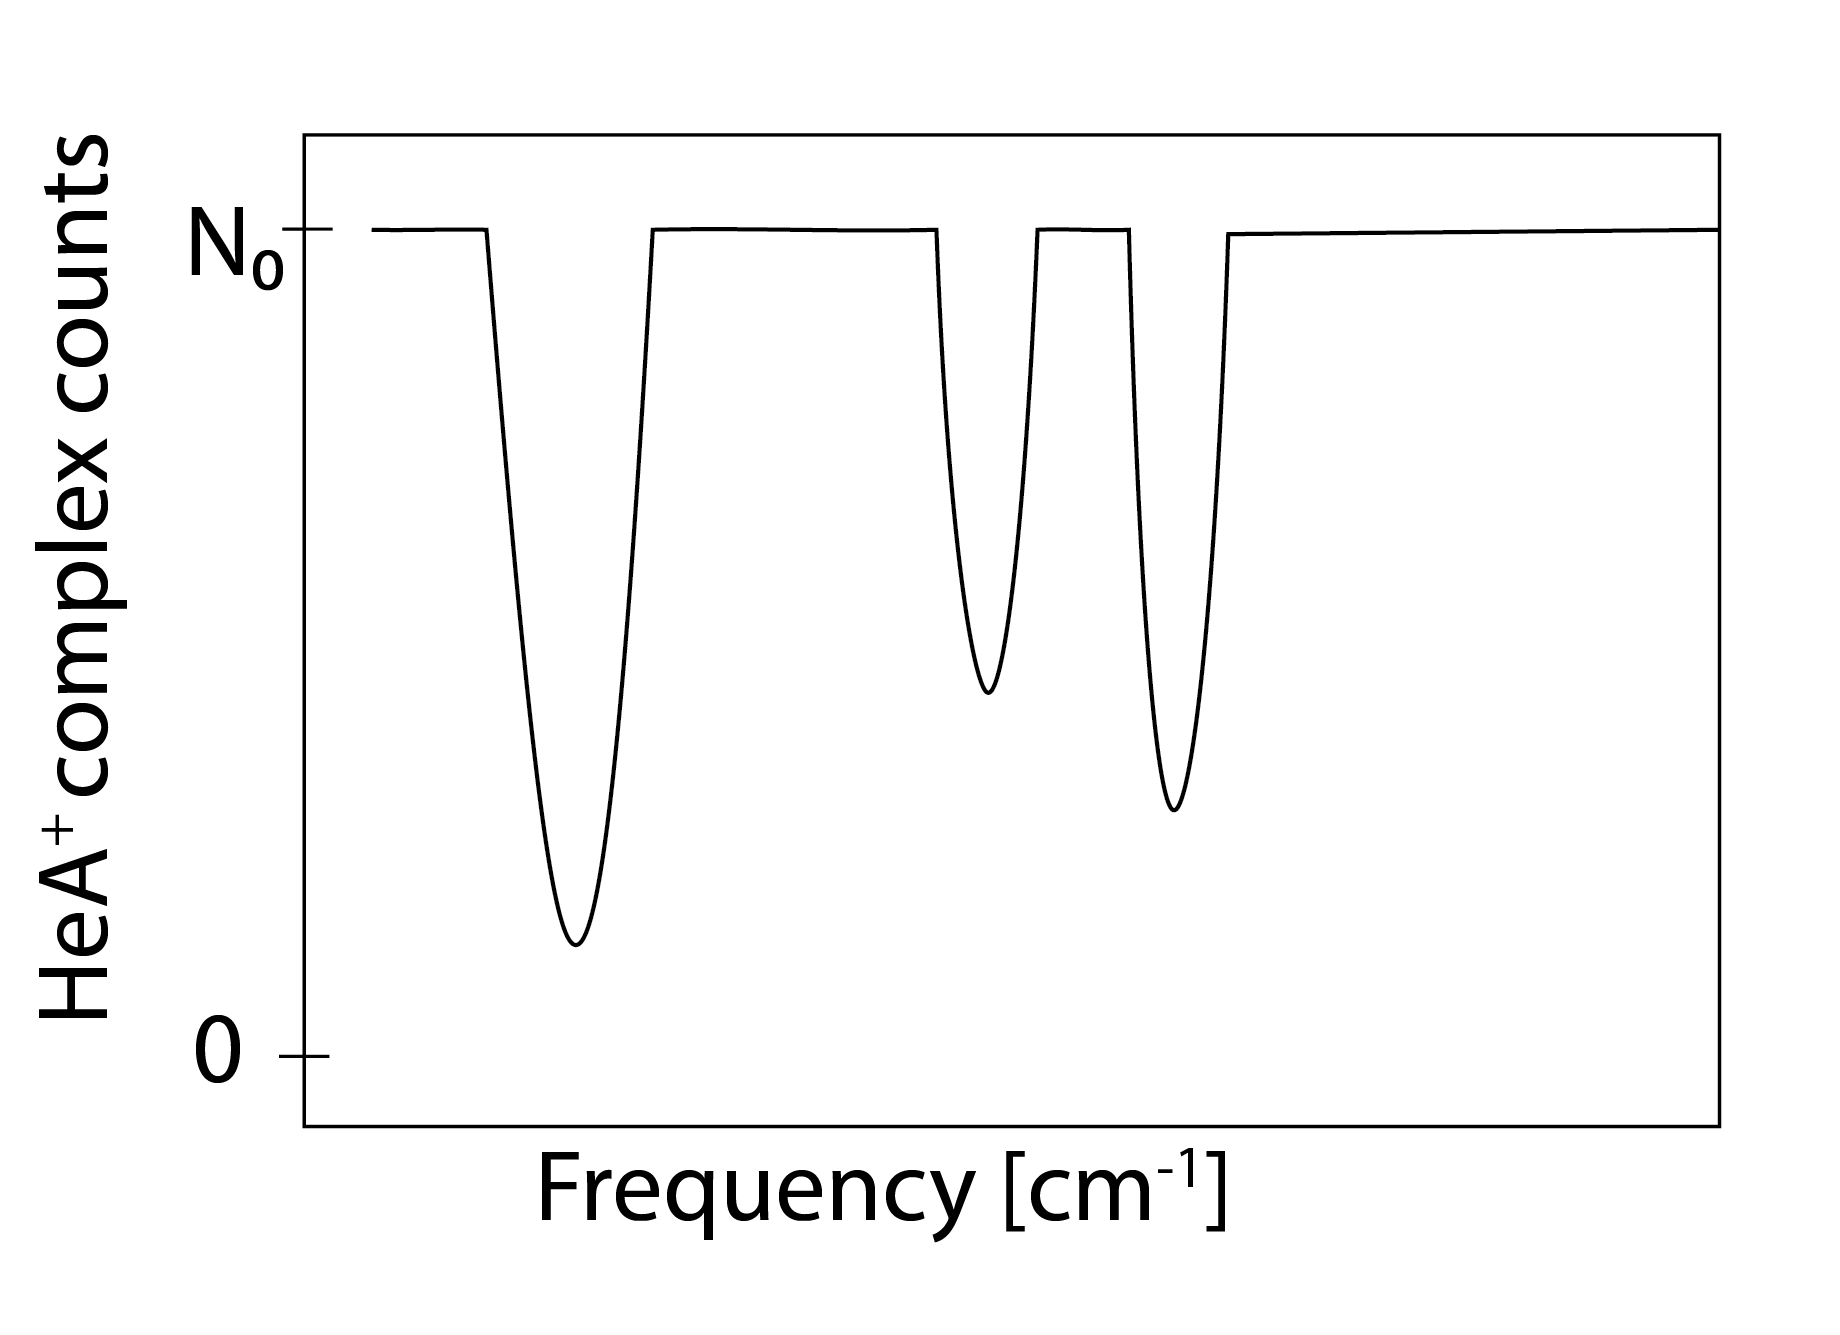
\includegraphics[scale=0.5]{figures/intro/IRPD_spectrum.png}
    \caption{Simulated IRPD spectrum measuring complex counts as a function of frequency. N$_0$ indicates the initial background counts, while the counts drop due to the dissociation of the complex at the resonance frequency.}
    \label{fig:IRPD_spectrum}
\end{figure}

Yuan T. Lee demonstrated the first  IRPD action spectroscopy technique  \cite{okumura_vibrational_1985} for hydrogen cluster ion, which several groups further developed \cite{bieske_spectroscopic_1993, duncan_infrared_2003, lisy_infrared_2006} using molecular beam experiments. However, in the molecular ion beam, the small interaction time between the ion and tag and ion and photons ( $\sim \mu$s range, flight time of ions) is a disadvantage for efficient complex formation and dissociation, respectively.
% Also, the ion sources synthesising weakly bound complexes often lead to vibrational hot bands.

Cryogenic ion trap experiments overcome these restrictions \cite{asmis_mass-selected_2002, kohguchi_high-resolution_2018, jusko_felion_2019, topfer_spectroscopic_2020, dahlmann_predissociation_2022} by storing for longer duration ($\geq 1$s) and by using cryogenic cooling to relax the molecular ion to its vibrational and electronic ground state. The low temperatures in the ion trap ($> 4$ K) also result in a high tagging efficiency even for weakly bound complexes \cite{roithova_helium_2016, gerlich_infrared_2018}, which is an important factor since the tagging method is predicated on the notion that the binding of the tag does not significantly alter the structure of the original ion. Consequently, the spectra produced from tagging spectroscopy can be correlated with the structure of "bare" ions.\\

The IRPD technique is employed in this thesis to characterize vibrational transitions of the molecular ion. Section \ref{sec:methods:vibration} discusses the integration of this technique into our 22-pole cryogenic ion trap instrument (Section \ref{sec:felion}). The following sections discuss several other methods developed for vibrational action spectroscopy in cryogenic ion traps.

\subsubsection{IR multi-photon dissociation (IRMPD)}
\label{subsec:action:methods:vibrational:IRMPD}

As discussed above, the energy of a single infrared (IR) photon is insufficient to cause dissociation in the majority of untagged ions. However, numerous photons can be absorbed when employing high-power light sources. The combined sum of the absorbed energy thus overcomes the dissociation energy limit, as shown in Figure \ref{fig:IRMPD}.

In 1973, Isenor and coworkers \cite{isenor_co2_1973} were the first to notice this IRMPD effect when they exposed SiF$_4$ vapour to powerful CO$_2$ laser pulses. This study was quickly replicated in laboratories worldwide, and it was later shown that many different types of molecules could undergo infrared multiple-photon dissociation or isomerization \cite{wight_infrared_1981, gaumann_infrared_1990, peiris_infrared_1993}. However, it was not until the 1990's that widely tunable free electron IR laser sources with adequate pulse energies became available, launching a new infrared ion spectroscopy area. \citet{oomens_gas-phase_2000} and \citet{lemaire_gas_2002} demonstrated the potential of a widely tunable infrared free-electron laser (FEL) in the study of the IR spectroscopy of mass-selected ions in an ion trap. 

\begin{figure}[!htb]
    \centering
    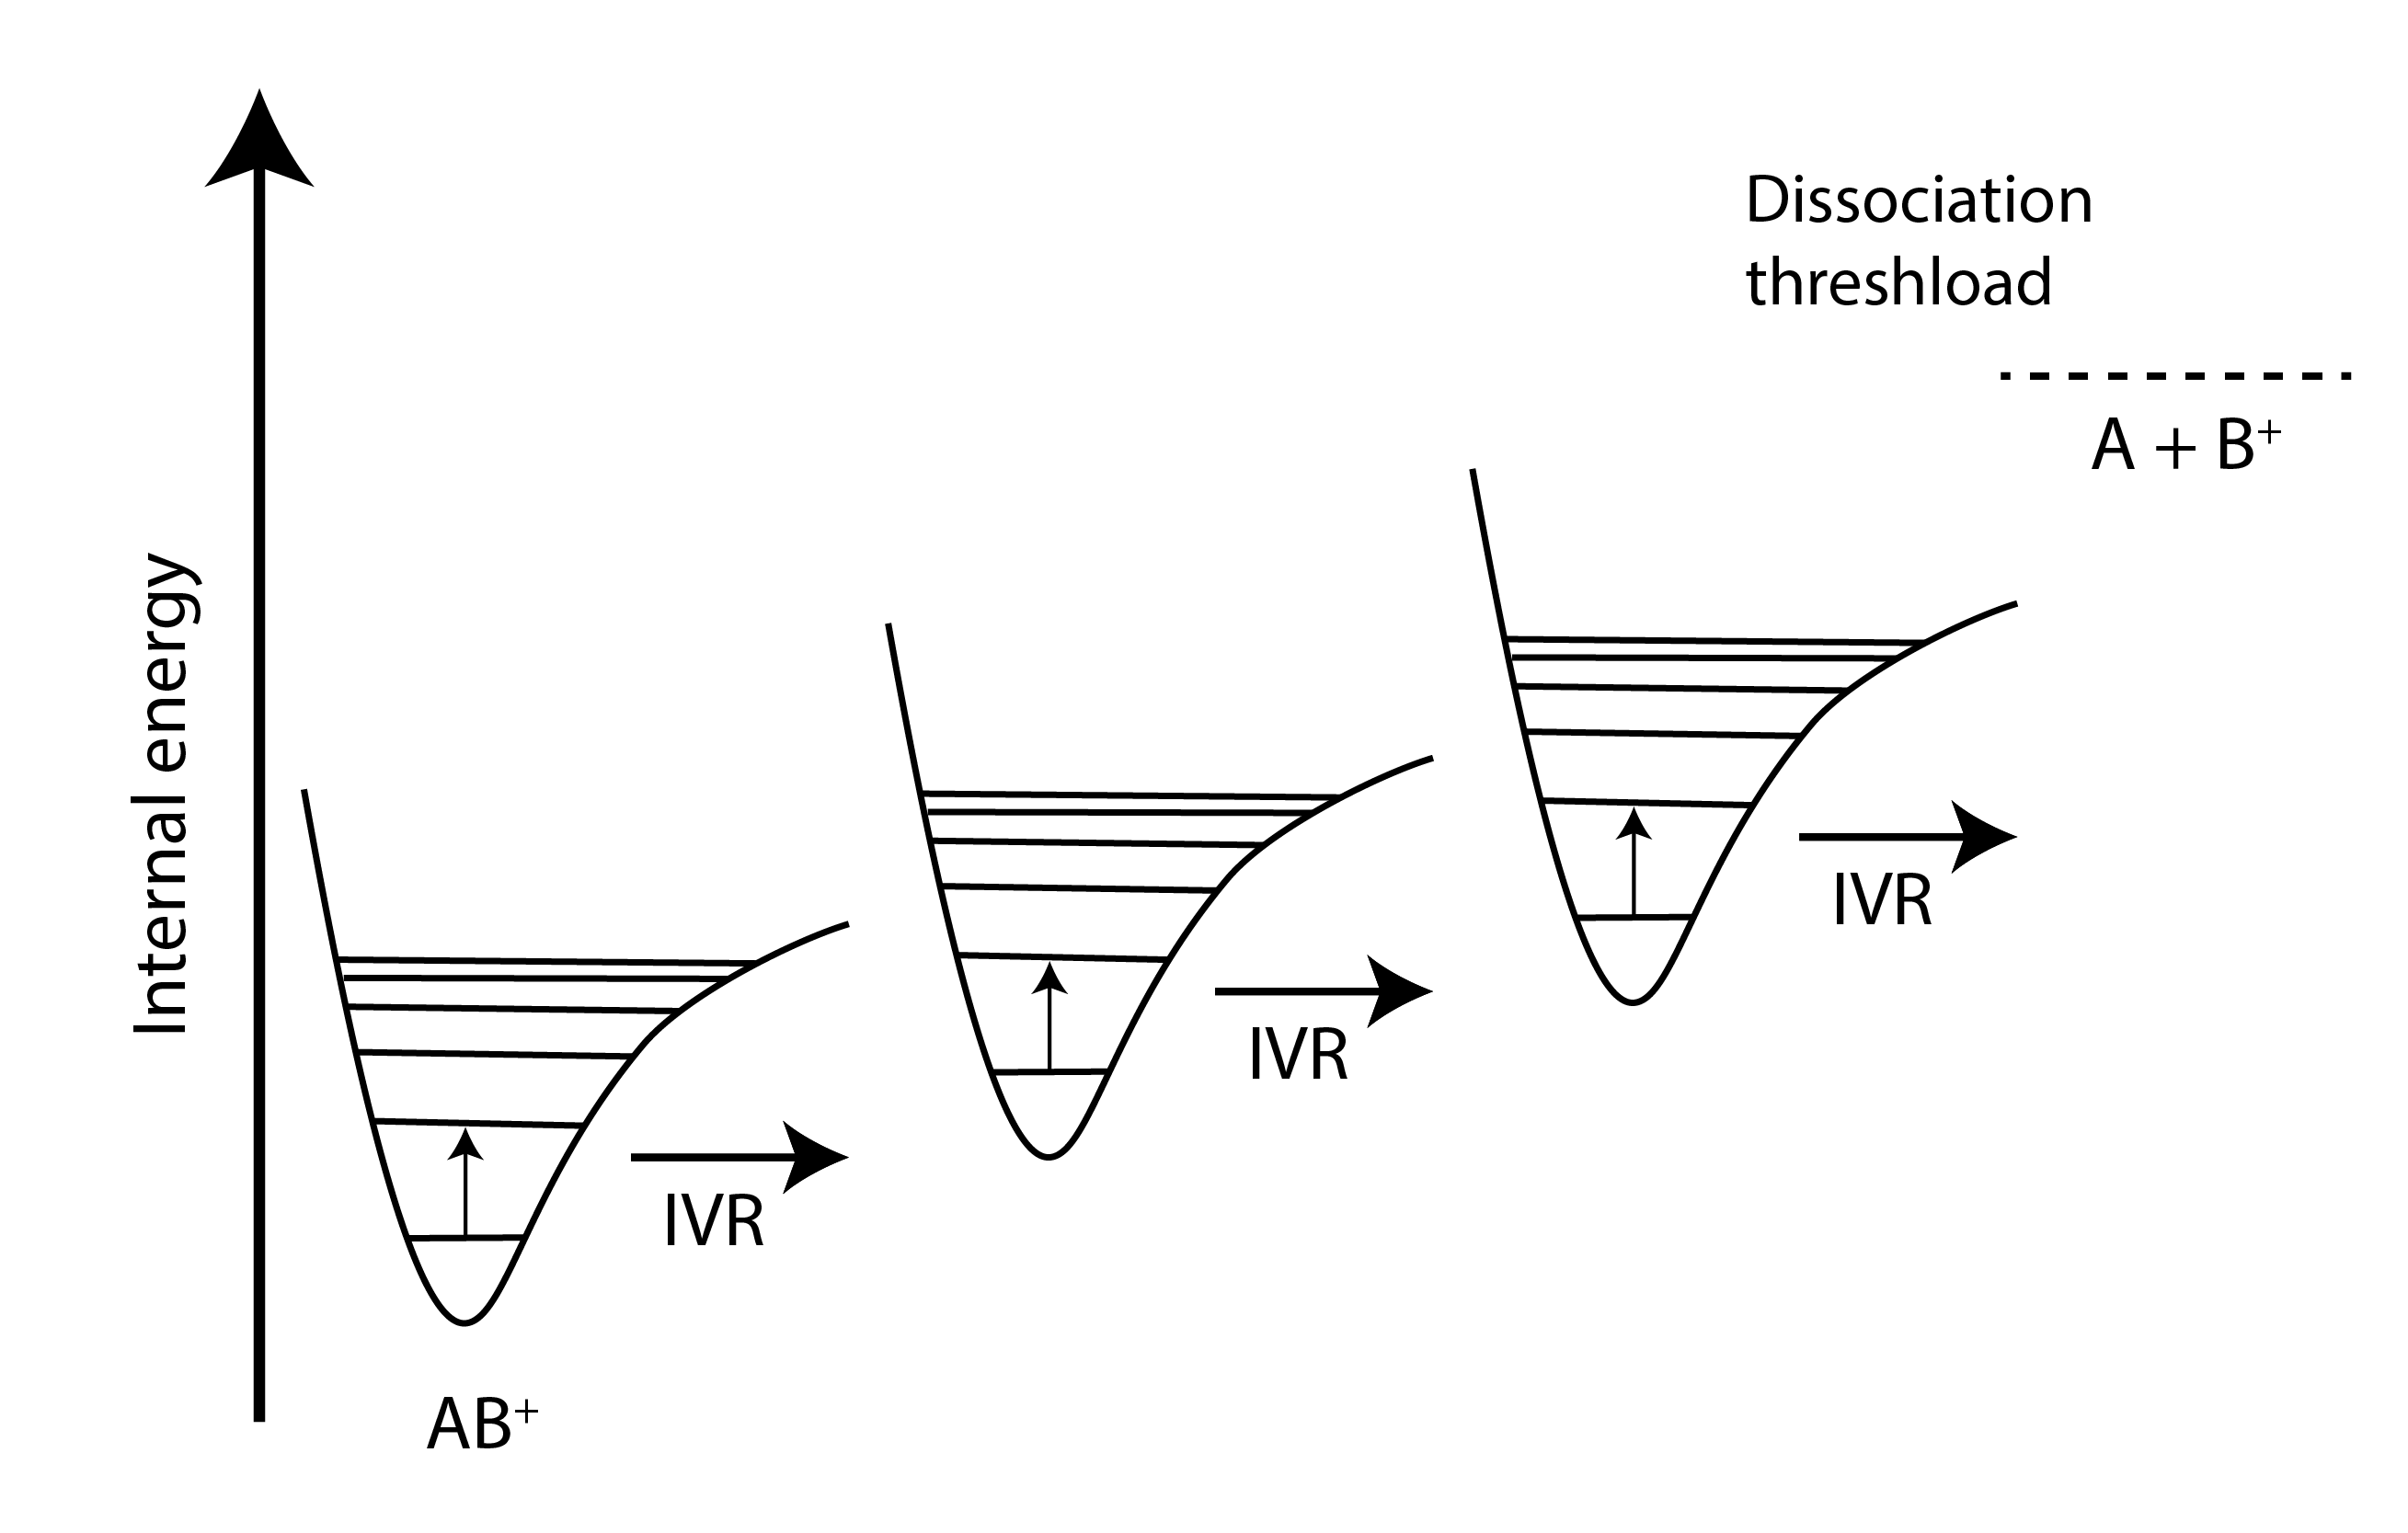
\includegraphics[scale=0.5]{figures/intro/IRMPD_IVR.png}
    \caption{Schematic drawing of the Infrared multi-photon dissociation (IRMPD) spectroscopy. AB$^+$ represents molecular ion consisting of A and B chemical fragments. Figure adapted from \cite{cpolfer_infrared_2011}.}
    \label{fig:IRMPD}
\end{figure}

Extensive experimental and theoretical research investigated the fundamentals of IR multiple-photon excitation in polyatomic molecules \cite{black_collisionless_1977, makarov_statistical_1998, oomens_gas-phase_2006, parneix_accurate_2013}. IRMPD is a low-energy fragmentation method that requires absorbing many photons of IR radiation before dissociation occurs. Vibrational potentials are inherently anharmonic, and absorption of tens to hundreds of photons occurs in a non-coherent manner. This effect is often referred to as the anharmonicity bottleneck \cite{steinfeld_molecules_1985}. Before the subsequent photon is absorbed, intramolecular vibrational redistribution (IVR) swiftly spreads the energy stored in the excited vibrational coordinate over all other vibrational degrees of freedom. The molecule is slowly heated, and dissociation typically follows the lowest-energy fragmentation pathway. 

However, this poses a difficult challenge to investigate small molecular ions using IRMPD because the method requires a high density of vibrational states, which guarantees that there are always a lot of vibrational eigenstates such that the IVR is feasible. Therefore IRMPD is typically well-suited for larger molecular ions. In this thesis, only smaller molecular ions ($\leq 7$ atoms) are investigated; hence IRPD is employed, as mentioned in the previous section.
% The other major disadvantage of IRMPD over IRPD is the broadening and shifting of the bands due to anharmonicity.

\subsubsection{Laser induced reactions (LIR)}
\label{subsec:action:methods:vibrational:LIR}

LIR combines the benefits of trapping molecular ions in a cryogenic ion trap with the idea of using a chemical reaction to determine the ion's internal state. In the late 1990s, \citet{schlemmer_laser_1999} developed LIR for spectroscopy by measuring the vibronic N$_2^+$ (A $ ^2\Pi_u \leftarrow$ X $^2\Sigma_g$) spectrum by excitation with visible laser photons to overcome the endothermic energy of a charge-transfer (CT) reaction as shown in equation \ref{eq:LIR:CT}. Counting the laser-induced product ions as a function of laser frequency yields the spectroscopic signal (see Figure \ref{fig:action:methods:vibrational:LIR-full}).

\begin{align}
    \text{N}_2^+ + \text{Ar} \rightarrow \text{Ar}^+ + \text{N}_2 \label{eq:LIR:CT}\\
    \text{C}_2\text{H}_2^+ + \text{H}_2 \rightarrow \text{C}_2\text{H}_3^+ + \text{H} \label{eq:LIR:H2_abstraction}\\
    \text{CH}_5^+ + \text{CO}_2 \rightarrow \text{CH}_4 + \text{OCOH}^+  \label{eq:LIR:proton_transfer}
\end{align}

\begin{figure}[!htb]
    \centering
    \Subfigure{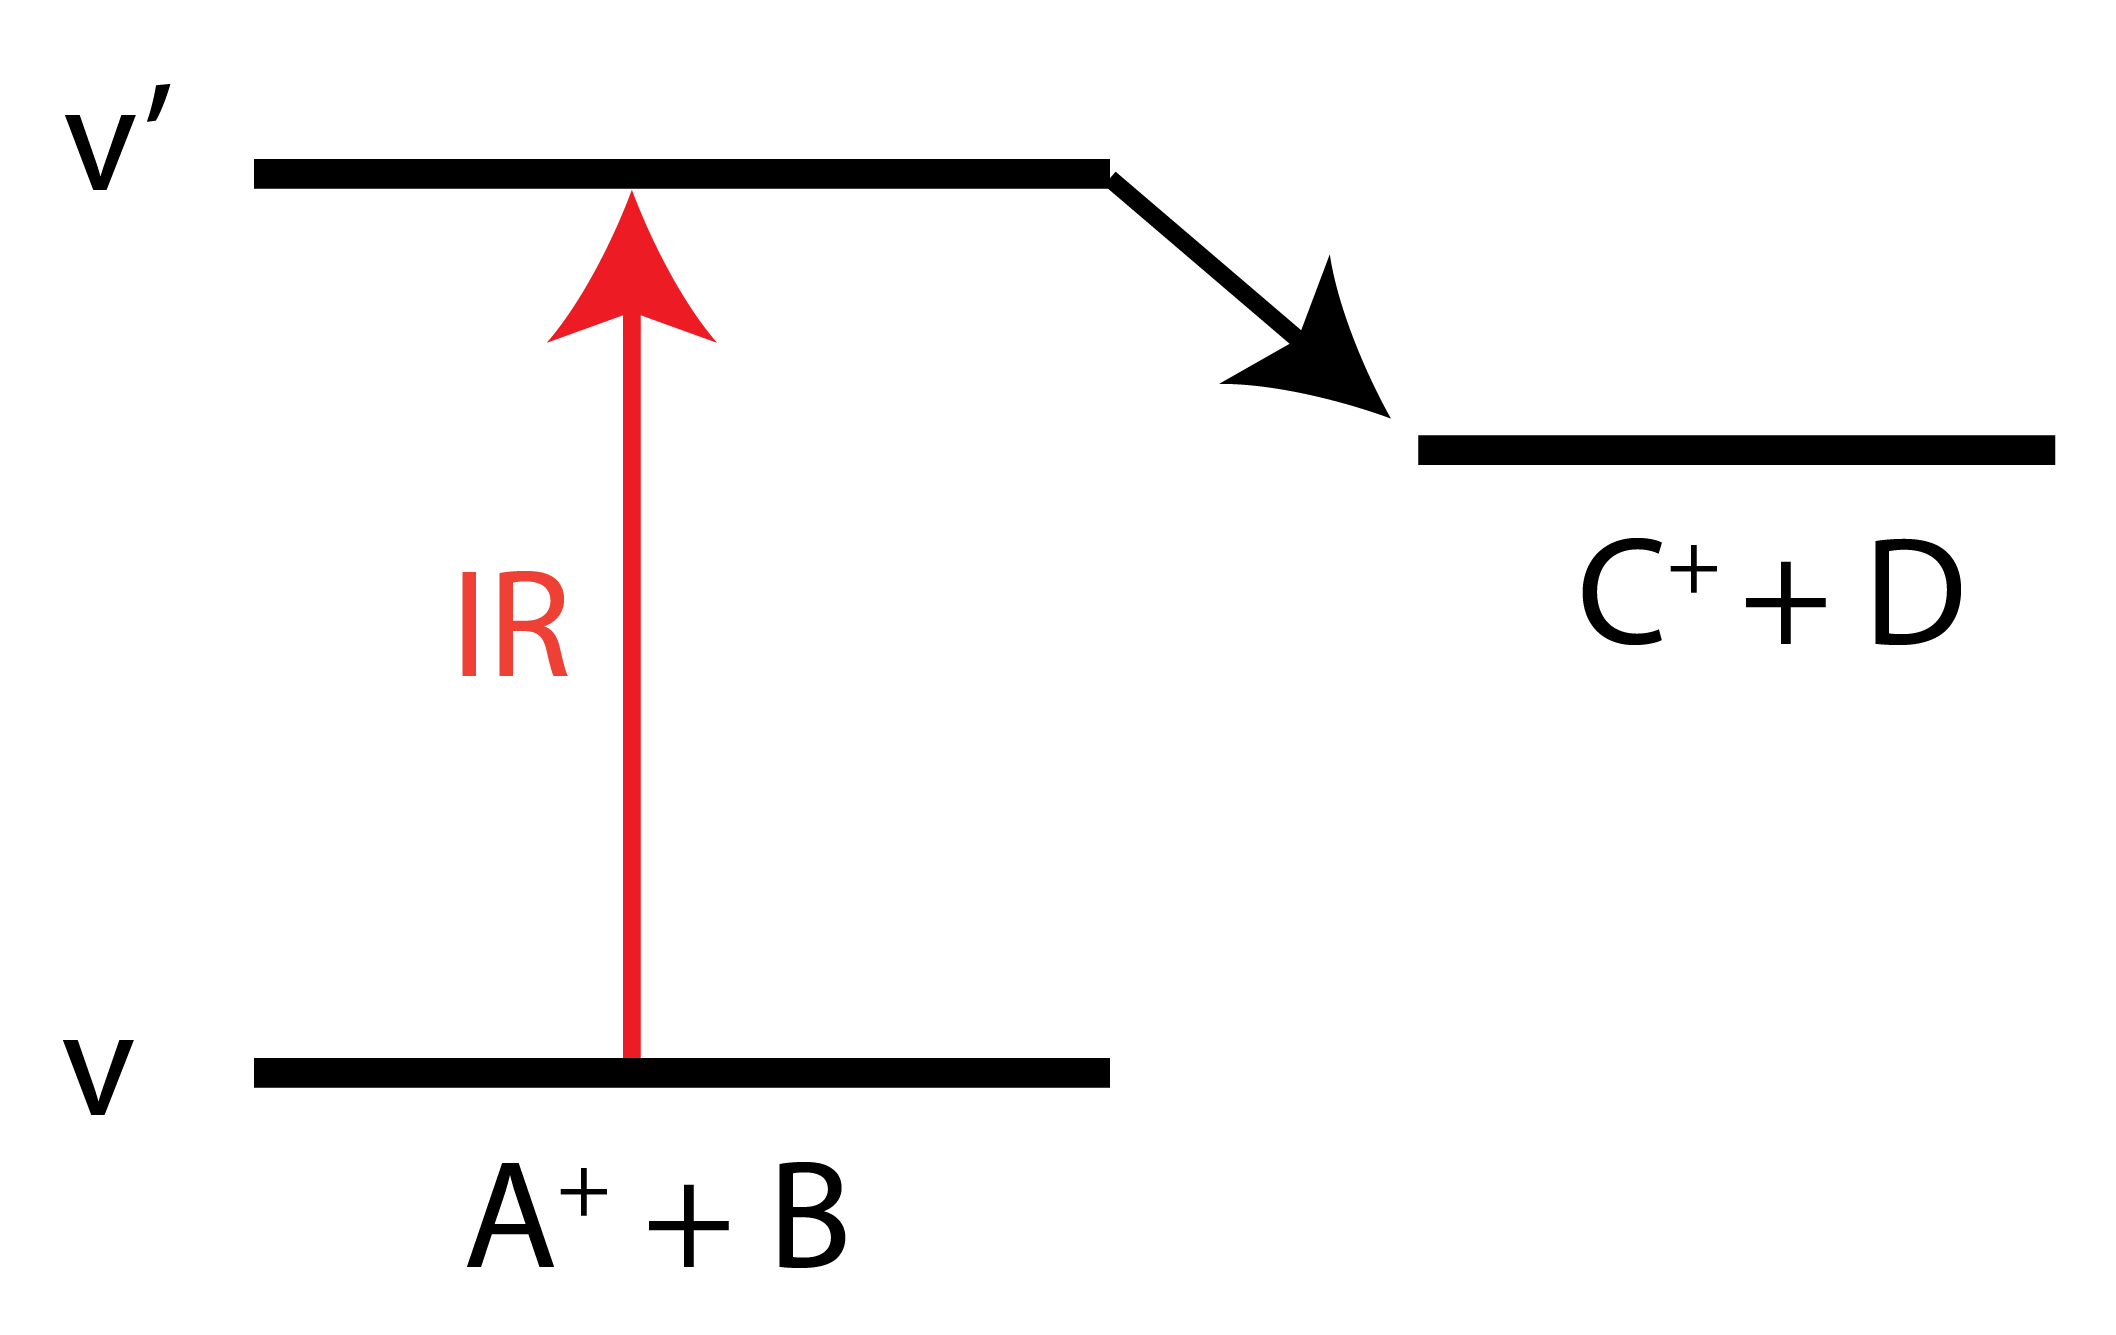
\includegraphics[width=1\textwidth]{figures/intro/LIR.png}}{}
    \hfill
    \Subfigure{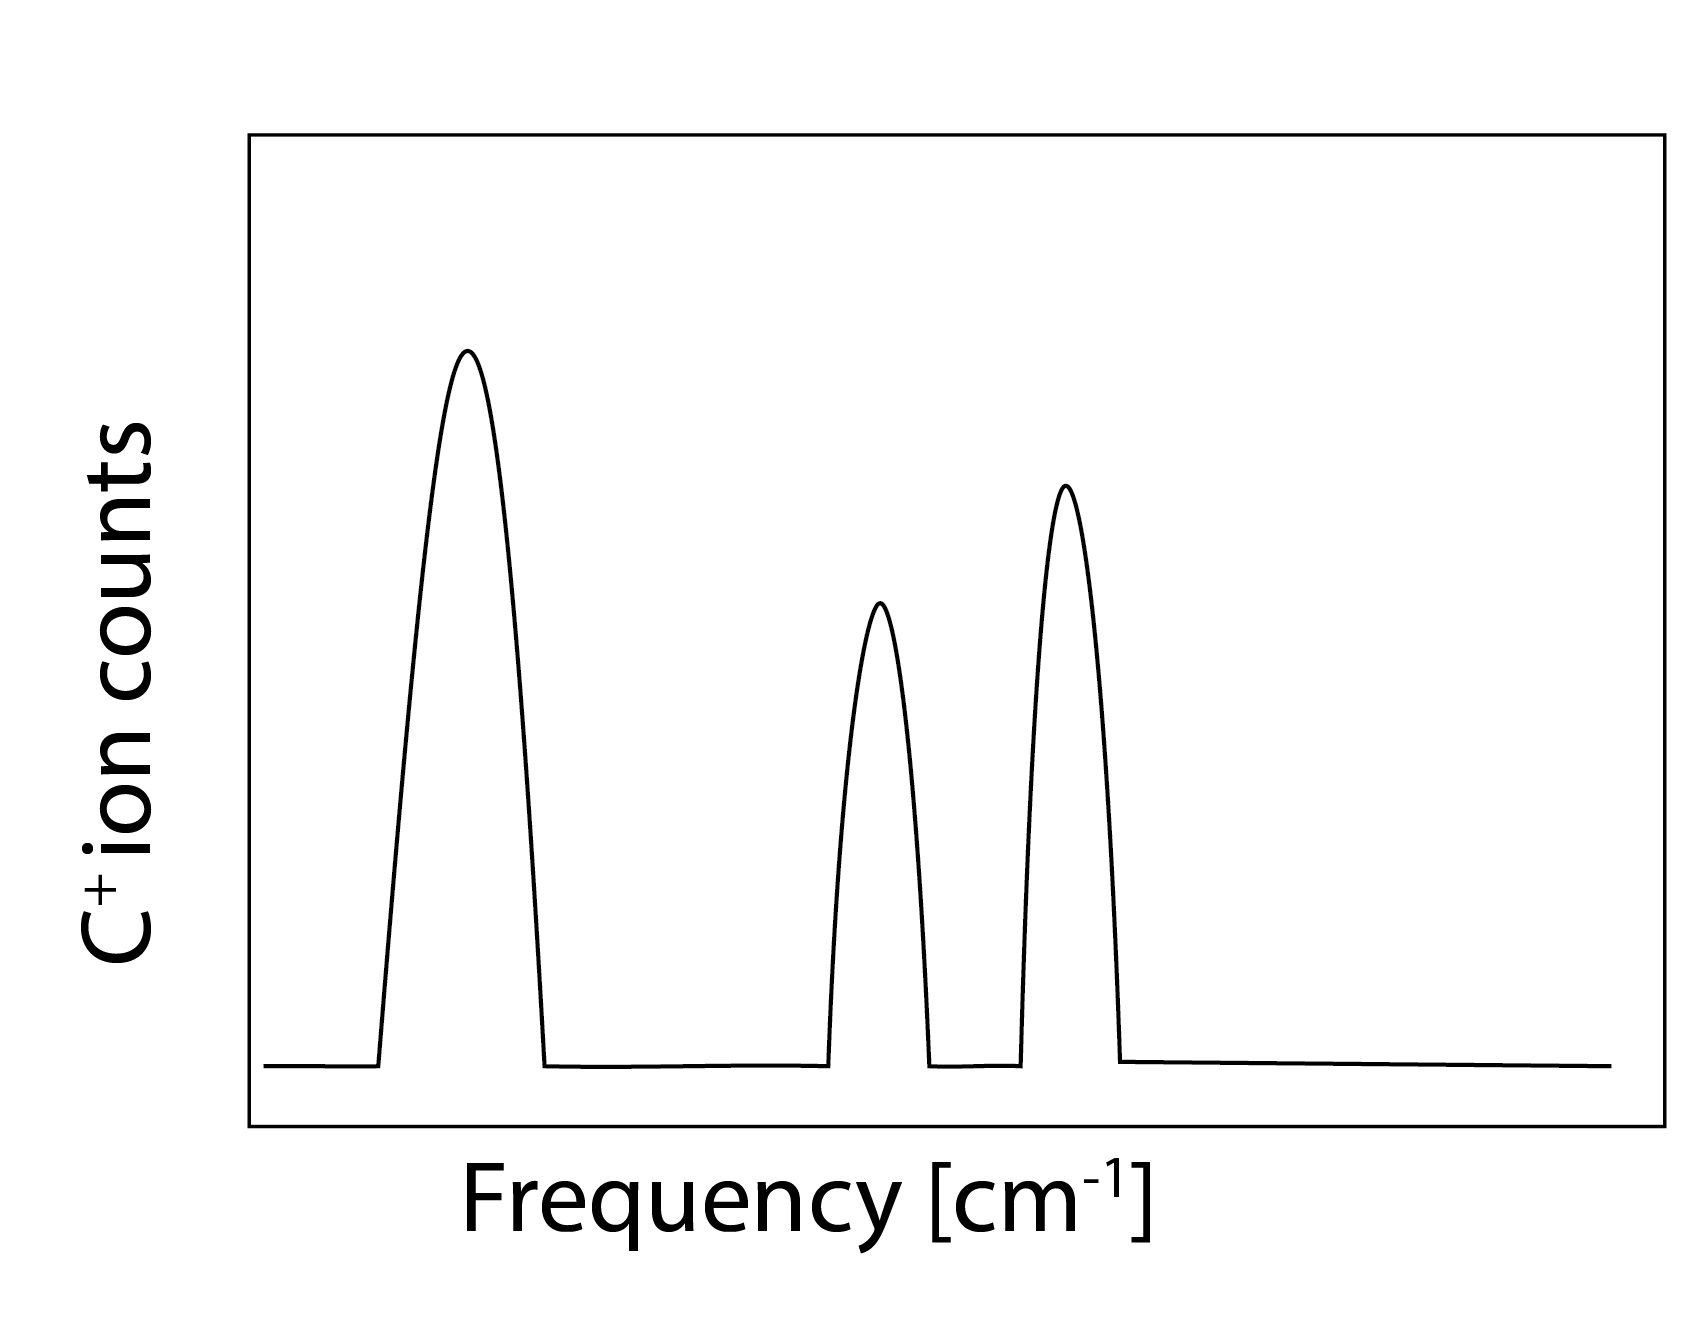
\includegraphics[width=1\textwidth]{figures/intro/LIR_spectrum.png}}{}
    \hfill
    \caption{Schematic description of (a) bimolecular reaction initiated by laser excitation suitable for LIR spectroscopy, (b) LIR signal as a function of frequency detected by monitoring the product counts.}
    \label{fig:action:methods:vibrational:LIR-full}
\end{figure}

Several endothermic reaction systems have been studied with the LIR method for bimolecular reactions, such as hydrogen abstraction and proton transfer (see Eq. \ref{eq:LIR:H2_abstraction} and  \ref{eq:LIR:proton_transfer}), to record vibrational transitions of reactant C$_2$H$_2^+$ \cite{schlemmer_laser_2002, asvany_experimental_2005, schlemmer_comparison_2005} and CH$_5^+$ \cite{asvany_understanding_2005}, respectively, by detecting the laser-induced products C$_2$H$_3^+$ and OCOH$_2^+$, respectively.

\subsubsection{Laser induced inhibition of He attachment (LIICG)}
\label{subsec:action:methods:vibrational:LIICG}

The requirement for an endothermic chemical reaction with a neutral reaction partner is an obvious limitation of the LIR method. Acquiring endothermic energy for chemical reactions is challenging, especially for highly reactive molecular ions. Also, the endothermicity cannot be too high since it needs to be overcome by the absorption of a single infrared photon. Another limitation is that since the cryogenic trap has very low temperatures, the neutral reaction partner should not condense in the trap. These conditions limit the use of LIR.

LIICG takes advantage of the fact that the excitation of molecular ions can inhibit the ternary attachment of He atoms. Maier and Gerlich \cite{chakrabarty_novel_2013} pioneered this method by measuring the electronic transition of N$_2^+$ (A $ ^2\Pi_u \leftarrow$ X $^2\Sigma_g$) using a 22-pole cryogenic ion trap.

First vibrational LIICG was demonstrated for rovibrational transitions in the floppy CH$_5^+$ molecular ion by \citet{asvany_coltrap_2014} by forming CH$_5^+-$He complexes and observing an on-resonance decrease in the number of CH$_5^+-$He due to laser-induced inhibition of helium attaching to CH$_5^+$ (not via destruction of CH$_5^+-$He as in IRPD). The vibrational LIICG has been employed to record many other molecular ions such as O$_2$H$^+$ \cite{kohguchi_high-resolution_2018}, CH$^+$ \cite{domenech_first_2018}, H$_3^+$, H$_2$D$^+$ and D$_2$H$^+$ \cite{jusko_frequency_2016}, CD$_2$H$^+$ \cite{jusko_high-resolution_2017}, CH$_2$NH$_2^+$ \cite{Markus2019}, CN$^+$ \cite{domenech_high-resolution_2020}; HHe$_2^+$ and HHe$_3^+$ \cite{topfer_spectroscopic_2020}.

Interestingly, the ternary rate coefficient for He attachment can be affected by rotational excitation, even though rotational photons only carry a fraction of energy compared to vibrational photons. Section \ref{subsec:action:methods:rotational:ROSAA} describes how to use this phenomenon to our advantage to measure high-resolution molecular ions' rotational spectra.

% \subsubsection{Double resonance methods}
% \label{subsec:action:methods:vibrational:DR}

% Double resonance spectroscopy uses two spectroscopic light sources simultaneously, often at very different wavelengths. Because of availability of different combination of lasers, there are several methods developed to study conformer/isomer selective studies. Only few techniques invlolving IR and UV lasers are discussed here as an example in this section.\\

% The technique of infrared–ultraviolet (IR–UV) double resonance (DR) spectroscopy has proven to be an effective method for the measurement of the conformation-selective vibrational spectra of polyatomic molecules, ions, and their clusters. The method involves using an IR laser pulse to change the molecule's vibrational population, followed by a UV laser pulse to detect this variation.\\

% \textbf{IR-UV depletion spectroscopy: } In this double resonance spectroscopy, infrared (IR) and ultra-violet (UV) lasers are used. By locking the UV laser onto the specific electronic transition characteristic of the selected isomer. When an isomer absorbs an incoming IR photon, the ground vibrational state depopulates. This is measured as a decrease in the UV-induced photo-fragmentation signal, typically between 5\% and 50\% for IR laser pulses with an energy of 10 mJ \cite{stearns_conformation-specific_2007}. This depletion is recorded as a function of IR frequency to provide a isomer-specific IR spectrum. This technique can detect subtle differences between isomers.

% \textbf{IR-UV gain spectroscopy: }Ions are kept in their ground vibrational state by cooling them to cryogenic temperatures, which also minimizes the thermal broadening of the electronic transitions \cite{nagornova_exploring_2013}. Any isomer that absorbs an IR photon causes internal heating, which causes broaden and redshift of the corresponding electronic spectrum. The infrared photodissociation spectra of ions are recorded using these changes in the electronic absorption. The UV laser wavelength is adjusted to the red of the cold ion's lowest energy electronic transition, which prevents dissociation. The spectrum is recorded as a function of IR frequency and on-resonance the spectral broadening caused by IR photon absorption increases the dissociation (signal gain).\\

